\documentclass[runningheads, final]{comsis2}

\def\journalissue{Computer Science and Information Systems 00(0):0000--0000}
\def\paperidnum{https://doi.org/10.2298/CSIS123456789X}
\setcounter{page}{1}

%% Use this to show line numbers (and remove only in the final camera-ready version)
\usepackage[pagewise]{lineno}
\linenumbers

\usepackage{hyperref}
\usepackage{booktabs}
\usepackage{verbatim}
\usepackage{graphicx}
\usepackage{amsmath}
\usepackage{amssymb}
\usepackage{tikz}
\usepackage{algorithm}
\usepackage{algpseudocode}
\usepackage{amsmath}
\usepackage{amssymb}
\usetikzlibrary{shapes.symbols, shapes.geometric, positioning, arrows.meta}

\bibliographystyle{unsrt}

\title{Multiobjective optimization model for regime adjustment in crude oil production}
\titlerunning{Multiobjective optimization in crude oil production}

\author{
    Matías Micheletto\inst{1} \and 
    Javier Marenco \inst{2} \and 
    Carlos De Marziani \inst{1} \and 
    Rodrigo Santos \inst{3}
}

\institute{  Instituto Multidisciplinario para la Investigación y el Desarrollo Productivo y Social de la Cuenca Golfo San Jorge - CONICET\\
            8000 Comodoro Rivadavia, Argentina\\
            \email{matias.micheletto@uns.edu.ar, cdemarzi@gmail.com}
            \and
            Universidad Torcuato di Tella\\
            C1428, Ciudad Autónoma de Buenos Aires, Argentina\\
            \email{javier.marenco@utdt.edu}
            \and
            Dep. Ing. Eléctrica y Computadoras, Universidad Nacional del Sur,
            8000, Bahia Blanca, Argentina\\
            \email{ierms@uns.edu.ar}
            }
\begin{document}
\maketitle

\begin{abstract}
    %A production battery in the oil industry is a set of equipment and facilities used in the initial stages of crude oil processing at an oilfield. At various stages of operation, it may be necessary to restrict or increase its processing capacity, meaning that the gross volume to be received must be adjusted. In remote areas where connectivity and infrastructure may be limited, it is necessary for an operator to approach the well in person to make manual adjustments directly to the pumping system. Proper planning of the well route for adjusting regimes directly impacts the operating costs of the oilfield. In this work in progress, a mixed integer linear programming model for this problem is proposed, by considering the production, operation, and modification restrictions of the pumping regime of each well. Preliminary results are presented, which show that the model can be used in practice. In mature conventional basins, production is typically organized through multiple batteries that deliver their output to a crude oil treatment plant. Within the framework of the industry’s digital transformation processes, these systems increasingly rely on supervisory and data acquisition platforms that enable remote monitoring of operational variables. However, certain control actions and adjustments of pumping systems still require the on-site intervention of specialized maintenance teams. These teams serve multiple batteries within an oilfield and must travel between wells to adjust pumping regimes in response to changes in the processing capacity of the treatment plant, maintenance activities, or operational constraints. In this context, planning field interventions becomes a relevant operational problem, in which production targets, process-related losses, and logistical travel costs must be considered simultaneously. Thus, this paper proposes a mixed-integer linear programming model to support decision-making in the adjustment of production regimes in oilfield batteries. The model integrates production and operational constraints with the planning of maintenance team routes, aiming to balance production goals with the minimization of losses and field intervention costs. Preliminary results indicate that the proposed approach is feasible and suitable for application under real operating conditions.
    
     In mature conventional oilfields, production is organized through geographically distributed batteries that operate under limited processing capacity. Although supervisory platforms enable remote monitoring, adjustments in pumping regimes frequently require on-site intervention by maintenance teams, whose movements generate significant logistical costs. Consequently, production reconfiguration decisions are intrinsically coupled with routing decisions, giving rise to a structured multiobjective optimization problem. This paper proposes a multiobjective mixed-integer linear programming (MILP) formulation that integrates production regime adjustment with maintenance team routing. The model simultaneously minimizes travel distance, production losses, intervention costs, and the number of adjusted wells, while satisfying battery capacity constraints. Intervention costs are modeled through operational risk and technical priority components, introducing realistic trade-offs between production importance and field intervention effort. Synthetic instances inspired by statistical properties of mature oilfields are generated to evaluate the computational performance of the formulation. Preliminary computational experiments illustrate the feasibility of the approach and the structure of the Pareto frontier, highlighting the trade-offs between operational efficiency and intervention costs.
      
    \vspace{6pt}
    \textbf{Keywords: }
    Oil \& Gas, 
    Multiobjective Optimization, 
    Mixed-Integer Linear Programming, 
    Production Routing, 
    Field Intervention Planning.
\end{abstract}

\section{Introduction}

%The Paris Agreement \cite{agreement2015paris} and the global transition toward lower-carbon energy systems have reshaped investment strategies within the oil and gas industry. 
The increasing pressure to improve efficiency in hydrocarbon production has reshaped operational strategies within the oil and gas industry. While non-conventional resources such as shale oil and shale gas have gained increasing prominence, mature conventional fields continue to play a significant role in energy supply. In these environments, the main challenge is not expanding production capacity,y but improving operational efficiency under limited processing and intervention resources \cite{SIRCAR2021379}. Mathematical programming approaches have been widely applied in oil production optimization, including mixed-integer and nonlinear formulations for production allocation and artificial lift systems  \cite{doi:10.1021/ie034171z}. 
%Advances in oil and gas exploration and production technologies have enabled the large-scale development of non-conventional resources, such as shale oil and shale gas, which in many regions have gained prominence over conventional production methods. As a result, non-conventional fields have attracted increasing investment and technological innovation, reshaping production strategies within the industry. As investment and technological development increasingly concentrate on non-conventional assets, mature conventional fields face the challenge of remaining economically viable by focusing on operational efficiency and cost optimization. New technologies applied to the exploration and extraction of oil and gas have allowed the development of fracking that has overpassed conventional methods. In Argentina, oil companies are leaving conventional wells and moving to Vaca Muerta, a region that is among the five largest shale oil and gas fields in the world. %In mature conventional fields, the main challenge does not lie in expanding production, but rather in adjusting operating costs and optimizing existing resources \cite{SIRCAR2021379}. 
%A production battery in the oil industry is a set of equipment and facilities used in the initial stages of crude oA production battery consists of facilities located near the wells, where extracted fluids are separated into oil, gas, water, and other components before being transported to treatment plants.l processing at an oilfield, within the \textit{upstream} sector. 

In mature conventional oilfields, production is typically organized through multiple batteries that collect and process the output of geographically dispersed wells before delivering it to a treatment plant. A production battery consists of facilities located near the wells, where extracted fluids are separated into oil, gas, water, and other components before being transported to treatment plants. Subsequently, oil and gas are transported to a treatment plant, distribution centers, or refineries through pipelines or tanker trucks. Figure \ref{fig:deploy} shows schematically the hierarchy of a conventional oil field production elements.

\begin{figure}
    \centering
    \input{jerarquia}
    \caption{Oil field hierarchy}
    \label{fig:deploy}
\end{figure}

%Although the commercial interest is oriented to fracking wells, there are still large mature conventional fields producing oil and gas. %A production battery in the oil industry is a set of equipment and facilities used in the initial stages of crude oil processing at an oilfield, what is known as \textit{upstream} sector. These are closed to where  wells are drilled and receive the extracted product for its processing and separation of oil, natural gas, water and other elements not useful. Both oil and gas are then stored for its transportation through pipelines or tanker trucks towards distribution centers or refineries.
%The gross production arriving at the well battery contains a certain proportion of crude oil and other fluids such as water, gas, and impurities. This proportion can vary from well to well and is usually referred to as yield. The difference between gross and net volume is called loss and is generally injected back into the well through appropriate mechanisms to maintain its relative pressure  \cite{HASSAN2023181}. Enhanced Oil Recovery (EOR), uses advanced techniques like injecting fluids (CO2, steam or chemicals) into depleted oil fields to boost production beyond primary (natural pressure) and secondary (water/gas flood) methods, by altering oil/reservoir properties to improve flow, significantly increasing total recovery. 

The gross production arriving at a battery contains varying proportions of oil, water, gas, and impurities, which determine the yield of each well. The difference between gross and net volume constitutes a process loss, which in many cases is reinjected to maintain reservoir pressure conditions\cite{HASSAN2023181} . Production batteries have limited processing capacity, usually expressed in barrels or cubic meters per day, which imposes operational constraints that require periodic adjustments to the production regimes of the associated wells.
Batteries, for their part, have a gross processing capacity that is typically measured in units of volume they can process per unit of time, such as barrels per day (BPD) or cubic meters per day ($m^3/d$). The net production is obtained from the result of this processing. A battery can process the volume generated by dozens of wells, or add the volume already processed from another battery. Operational events such as maintenance or downstream constraints may require adjusting the gross volume processed by a battery, which in turn forces modifications in the operating regimes of the associated wells. This involves increasing or decreasing the production volume extracted from the wells, which translates into adjusting the operating regimes of the pumping systems.

Digital transformation initiatives have progressively incorporated supervisory and data acquisition platforms that enable remote monitoring of operational variables\cite{BIST2024100256}. However, these monitoring systems do not eliminate the need for physical intervention. In many conventional oilfields, adjustments in pumping regimes still require on-site intervention by as valve configurations or pumping flow rates. These field movements introduce significant logistical costs and operational delays, particularly in geographically dispersed fields with limited infrastructure. Therefore, production decisions cannot be treated independently from field logistics. Consequently, production reconfiguration decisions are intrinsically coupled with routing decisions: modifying the operational regime of a well implies a physical visit by maintenance personnel.

From a modeling perspective, this situation gives rise to a structured optimization problem in which continuous production control variables must be coordinated with discrete routing decisions. This structural coupling resembles integrated production–routing problems studied in operations research, such as the Production Routing Problem \cite{doi:10.1287/ijoc.1100.0439} and the Inventory Routing Problem \cite{Bertazzi2008} , where operational and logistical decisions are optimized simultaneously. In contrast, classical formulations focus on goods distribution and inventory management, whereas the problem addressed here involves endogenous routing decisions triggered by continuous operational regime adjustments.

%Conventional oil fields in Argentina are in south Patagonia mostly with sparse or no connectivity at all. The configuration set up of the wells should be performed by a worker that actually moves among the different wells. This movement has a cost both in money and time.  
%To meet the requirements arising from the change in gross production volume, production operations engineers must select the wells whose operating regimes need to be changed and calculate the new production parameters. This must be done taking into account the cost of modifying the operating regimes of each pumping unit. There is an optimization problem in this that has to complimentary objectives: i) the maximization of the oil production; ii) the minimization of the time or cost required to change the set up.
%The main contribution of this paper is the formalization of the problem through a mixed linear programming model that combines the optimization of well production subject to minimizing the distance traveled by the operator. This is achieved by combining linear programming and integer linear programming models. The model also incorporates a set of constraints related to the geographical location of the well site.

These interacting decisions naturally induce trade-offs between production efficiency and field intervention effort. Multiobjective vehicle routing problems have been extensively studied \cite{JOZEFOWIEZ2008293}, and structured mathematical programming approaches such as the $\varepsilon$-constraint method provide systematic mechanisms for generating Pareto-efficient solutions in multiobjective mixed-integer models \cite{MAVROTAS2009455} \cite{10.1007/978-3-319-15892-1_8}. However, despite advances in multiobjective routing and production planning, the explicit integration of production regime adjustment with maintenance routing under a unified multiobjective mixed-integer linear programming (MILP) framework remains largely unexplored in the context of conventional oilfield operations where routing is triggered by operational regime modification decisions.In this context, this paper proposes a multiobjective MILP formulation that integrates:

\begin{itemize}
    \item Production regime adjustment under battery capacity constraints;
    \item Maintenance team routing across geographically dispersed wells;
    \item Minimization of production losses derived from gross–net differences;
    \item Intervention cost modeling based on operational risk and technical priority.
\end{itemize}

The proposed model captures the structural interaction between production efficiency and field logistics within a unified optimization framework. Synthetic instances inspired by statistical characteristics observed in mature conventional oilfields are generated to evaluate the computational behavior of the formulation under controlled and reproducible conditions. The main contributions of this work are:
\begin{itemize}
    \item A unified multiobjective MILP formulation capturing the endogenous interaction between production regime adjustment and maintenance routing;
    \item A multiobjective structure balancing production efficiency and field intervention costs;
    \item A statistically grounded instance generation framework for reproducible experimentation;
    \item A computational analysis illustrating trade-offs between production losses and logistical costs.
\end{itemize}

%The main contribution of this work is the formulation of this problem through a mixed-integer linear programming model that integrates the optimization of production regimes with the planning of maintenance team routes. The model incorporates production, operational, and geographical constraints, and supports decision-making in conventional production environments that seek to maintain competitiveness through operational efficiency and digitalization.

The rest of the paper is organized as follows. Section 2 reviews related work. Section 3 presents the problem description. Section 4 details the MILP formulation. Section 5 describes the synthetic instance generation procedure. Section 6 reports computational results. Finally, Section 7 concludes the paper and outlines future research directions.
\section{Previous work} \label{sec:previos} 

The problem addressed here is related to the exploitation of hydrocarbons, particularly the oil industry in Argentine Patagonia. No works have been found that address the problem exactly as described here; therefore, some works with similar aspects are listed below.

In \cite{aronofsky1962,hartsock1971}, the importance of applying optimization methods and developing operational research strategies in the oil industry is introduced, within the context of limited operating resources and during a period of significant industry growth.

In \cite{duhamel2009multicommodity}, the authors present the "Mobile Oil Recovery" problem for the Petrobras company. This involves obtaining oil by pumping from a mobile unit (truck) that extracts from a field with low-yield wells. The optimization problem consists of maximizing extraction while reducing costs. The paper proposes the problem with a single pumping unit or with several. The proposed solution was tested with up to 200 wells in the battery. The fundamental difference with the present work is that this does not involve a mobile extraction unit, but the operator must travel through the well network to adjust the production parameters of each one according to the calculated optimal value.

In \cite{langvik2012optimization}, an optimization model for oil production on offshore platforms is presented. The objective of the work is to maximize oil extraction, considering the yield in relation to the water, crude oil, and gas extracted from each well, as well as the storage and routing of the generated flows. A linearization of the model is performed using mixed-integer linear programming techniques.

This work combines the optimization of the working regimes of the well battery to obtain a net production, minimizing loss on one hand and the path the operator must travel to reconfigure the wells on the other. During the bibliographic survey recently conducted by the authors, no model proposals like the one presented in this work have been found.
\section{Problem description} \label{sec:form}

Let ${\cal B} = \{1,\dots,B\}$ be the set of production batteries and let $\mathcal{W}=\{1,\ldots,W\}$ be the set of wells. Each battery $t\in {\cal V}$ groups a set ${\cal W}_t \subseteq {\cal W}$ of wells. Each well $W_i$ is described by the tuple $(G_i,N_i,r_i)$, where $G_i$ is the oil gross volume in $m^3/day$ produced, $N_i$ is the oil maximum net volume in $m^3/day$ produced, and $r_i \in (0,1)$ is the original well regime. We adopt the maximum values for the gross and net volumes produced since the actual production values are proportional to the regime ratio $r_i$. Although it is possible to assume $r_i$ as a continuos variable, in some cases it is restricted to just a few values determine by the technology used in the pumping. 

Let $t\in {\cal B}$. Once the battery gross production value $G'_t$ is set, the different wells should adjust their regime to satisfy the demanded value. For this, a new $r'_i$ has to be computed in such a way that:

\begin{equation} \label{eq:restr}
    G'_t = \sum_{i = 1}^{W} G_i \cdot r'_i.
\end{equation}

$G'_t$ is the objective value and as such is an input variable to the system determined by the engineers in charge of the production.

As explained before, most of the wells within a battery required the presence of an operator to set the appropriate regime that includes several aspects like opening/closing valves or setting pumping flow rate among other tasks. Usually workers are located within the operations center and from there they moved towards the different wells. For this they usually move with 4x4 trucks along dirty roads many times covered with snow or black ice. There is a cost associate both in time and resources to move along the wells. To incorporate this issue, an objective function is added with the total cost of the movements. For this purpose, the parameter $d_{ij}$ is defined, which models the cost, either in time or distance, of traveling from well $i$ to well $j$. A binary variable $x_{ij}$ that indicates whether wells $i$ and $j$ are visited consecutively by some operator is incorporated. In this way, the total cost $T$, which involves traveling between all the wells that must adjust their work regimes, is calculated according to the following equation:
\begin{equation} \label{eq:minT}
    T = \sum_{i = 0}^{W} \sum_{j = 0}^{W} d_{ij} \cdot x_{ij}.
\end{equation}
We assume that there are $\omega \in \mathbb{Z}_+$ operators, and this objective function considers the total travel distance of all of them. 

The second objective function is related to the cost associated to the loss in the production, mainly the difference between the gross and net volumes, $L_i$ It is computed by the following equation:

\begin{equation}
    L_i = G_i - N_i,
\end{equation}
Like in equation (\ref{eq:restr}), the total loss of the battery is $L'_t$ and is computed as:
\begin{equation} \label{eq:minL}
    L'_t = \sum_{i = 1}^{W} L_i \cdot r'_i.
\end{equation}
The optimization problem consist in minimizing at the same time the two objective functions (\ref{eq:minT}) and (\ref{eq:minL}) while satisfying the condition given in (\ref{eq:restr}).


% \skipthis{Esta restricción puede resultar limitante para la búsqueda de una solución óptima empleando algoritmos metaheurísticos como la optimización por enjambre de partículas (PSO), algoritmos genéticos (GA) o recocido simulado (SA). Sin embargo, al llevar el problema a la práctica se puede suponer un margen de error entre ambos valores, a modo de tolerancia, entre la producción bruta total y la obtenida al ajustar los nuevos regímenes de trabajo.

% Entonces el error $e_t$ obtenido al calcular el nuevo valor bruto total respecto del valor bruto deseado no debe superar un valor de tolerancia $E_t$, entonces se define un nuevo valor estimado $G'_{et}$ tal que,

% \begin{equation}\label{eq:tol}
%     G'_{et} = G_t \pm e_t, \;\; \text{con} \;\;\; e_t \leq E_t.
% \end{equation}

% Substituyendo la ecuación \ref{eq:restr} en la ecuación \ref{eq:tol} se puede expresar la nueva restricción como 

% \begin{equation} \label{eq:tol2}
% \left| G'_{et} - \sum_{i = 1}^{W} G_i \cdot r'_i \right| \leq E_t.
% \end{equation}
% }

The third objective function consists in minimizing the number of adjusted wells, while the fourth objective function is the sum of the costs associated with all the treated wells. To this end, let $C_i$ be the cost associated with the well $i$, for $i\in W$. The cost associated to a well is explained in what follows.
To model intervention costs more realistically, the cost parameter $C_i$ is decomposed into two components:

\begin{itemize}
    \item Operational Risk $R_i$
    \item Technical Priority $P_i$
\end{itemize}

Operational risk is assumed to increase with well productivity, as higher-output wells typically operate under greater mechanical stress. Accordingly, $R_i$ is generated as a function of normalized gross production:

\[
R_i = \rho_G \frac{G_i}{\max_j G_j} + \varepsilon_i^R,
\]

where $\rho_G$ is a scaling coefficient and $\varepsilon_i^R$ is a small zero-mean perturbation term.

Technical priority reflects strategic or reservoir-management considerations and is assumed to correlate with net production:

\[
P_i = \rho_N \frac{N_i}{\max_j N_j} + \varepsilon_i^P,
\]

where $\rho_N$ is a scaling factor and $\varepsilon_i^P$ is a perturbation term.

The intervention cost is then computed as:

\[
C_i = w_R R_i - w_P P_i + \kappa,
\]

\noindent where $w_R$ and $w_P$ are weighting coefficients and $\kappa$ is a positive constant ensuring non-negativity of costs. This formulation introduces realistic trade-offs between production importance and operational risk.
\section{ILP Model} \label{sec:modelo}
In this section, the ILP model is developed. For each well $i$, the continuous variable $r'_i \in [0,1]$ represents the new operational regime. A binary variable $z_i \in \{0,1\}$ is introduced to represent changes in the operation of the well in such a way that $z_i = 1$ when $r'_i \ne r_i$. For each pair of wells $i,j$, the binary variable $x_{ij}=1$ if some operator visits the well $j$ immediately after the well $i$. Well $0$ represents the battery operations center from which the operators begin their tours. Finally, the continuous value $y_i \in [0,W]$ is used to express through MTZ constraints the order in which the wells are visited. From these definitions the ILP model can be written as:

\begin{eqnarray}
\min & & \hspace*{-0.5cm} \sum_{i=0}^W \sum_{j=0}^W d_{ij} \; x_{ij} \label{obj.distancia} \\
\min & & \hspace*{-0.5cm} \sum_{i=1}^W (G_i - N_i) \; r'_i \label{obj.perdida} \\
\min & & \hspace*{-0.5cm} \sum_{i=1}^W C_i z_i \label{obj.costo} \\
\min & & \hspace*{-0.5cm} \sum_{i=1}^W z_i \label{obj.cantidad} 
\end{eqnarray}
\begin{eqnarray}
\sum_{i=1}^W G_i \; r'_i & = & G'_t \hspace*{1.57cm} \forall t\in {\cal B} \label{constr.target} \\
r'_i & \ge & r_i - z_i \hspace*{1.57cm} i=1,\dots,W \label{constr.ligarrwsuperior} \\
r'_i & \le & r_i + z_i \hspace*{1.57cm} i=1,\dots,W \label{constr.ligarrwinferior} \\
%\end{eqnarray}
%\begin{eqnarray}
\sum_{i=0}^W x_{ji} & = & z_i \hspace*{2.35cm} i = 1,\dots,W \label{constr.recorrer} \\
\sum_{i=1}^W x_{0i} & = & \omega \label{constr.salida} \\
\sum_{j=0}^W x_{ji} & = & \sum_{j=0}^W x_{ij} \hspace*{1.65cm} i=1,\dots,W \label{constr.flujo} \\
y_i + 1 & \le & y_j + W (1 - x_{ij}) \hspace*{0.2cm} i,j=1,\dots,W, \nonumber \\
        &     & \hspace*{2.65cm} i\ne j \label{constr.mtz} 
\end{eqnarray}        
\begin{eqnarray}
r'_i & \in & [0,1] \hspace*{1.95cm} i=1,\dots, W \label{constr.domrp} \\
z_i & \in & \{0,1\} \hspace*{1.8cm} i=1,\dots,W \label{constr.domz} \\
x_{ij} & \in & \{0,1\} \hspace*{1.8cm} i,j=1,\dots,W \label{constr.domx} \\
y_i & \in & [0,W] \hspace*{1.75cm} i=1,\dots,W \label{constr.domy}
\end{eqnarray}

There are four objective functions, minimizing the total distance (\ref{obj.distancia}), the total loss (\ref{obj.perdida}), the total cost (\ref{obj.costo}), and the number of adjusted wells (\ref{obj.cantidad}). Constraints (\ref{constr.target}) specify the total loss that should be obtained with the new regimes in the wells. Restrictions (\ref{constr.ligarrwsuperior}) and (\ref{constr.ligarrwinferior}) link the variables $r'$ and $z$ in such a way that $z_i=1$ if $r'_i\ne r_i$ (changes regime). Constraints (\ref{constr.recorrer}) specify that all the wells that change regime should be visited to adjust the production, that is all wells such that $z_i=1$. Restrictions (\ref{constr.salida}) state that the operators should begin the tour in the battery operation center (Well $0$), and the restrictions  (\ref{constr.flujo}) express the conditions for flow conservation at each well. Together with constraints of type MTZ, (\ref{constr.mtz}) these restrictions ask the variables $x$ to represent a hamiltonian circuit among the wells that change regime. Finally, restrictions (\ref{constr.domrp})-(\ref{constr.domy}) determine the variables' domains.


%In Figure \ref{fig:satelital} a small battery in the south of Argentina is represented with the roads connecting the different wells and the operation center.

% \begin{figure}[ht]
%   \centering
%   
\includegraphics[scale=0.2%width=0.47\textwidth
%   ]{caminos_sub_numerados.png}
%   \caption{Roads connecting wells in a small size battery in the south of Argentina obtained from satellite images. Location: 46$^\circ\text{40'50''S 67}$ $^\circ\text{51'29''W}$ (Santa Cruz, Argentina).}
%   \label{fig:satelital}
% \end{figure}

\section{Synthetic Instance Generation} \label{sec:instances}

To evaluate the proposed optimization model under controlled yet realistic operating conditions, synthetic instances were generated following statistical assumptions inspired by production behavior observed in mature conventional oilfields. The objective of this procedure is to reproduce key structural characteristics of real production systems while maintaining reproducibility and scalability.

For each well $i$, the maximum gross production $G_i$ (in $m^3/\text{day}$) is generated using a lognormal distribution. This choice reflects the empirical observation that well productivity in mature basins is strictly positive and typically exhibits right-skewed behavior, with a small number of high-performing wells and a majority of low-to-medium producers. Formally,

\[
G_i \sim \text{LogNormal}(\mu_G, \sigma_G),
\]

\noindent where parameters $\mu_G$ and $\sigma_G$ control the median production level and heterogeneity of the field, respectively. Increasing $\sigma_G$ produces instances with higher dispersion and greater optimization difficulty.


Net production $N_i$ is modeled as a fraction of gross production:
\[
N_i = \alpha_i G_i,
\]

\noindent where $\alpha_i \in (0,1)$ represents the effective recovery ratio. The parameter $\alpha_i$ is drawn from a Beta distribution:

\[
\alpha_i \sim \text{Beta}(a,b).
\]

The Beta distribution is selected due to its flexibility and bounded support. By choosing $a < b$, the distribution can be skewed toward lower values, representing high water-cut conditions commonly observed in mature conventional fields.


The initial regime $r_i \in (0,1)$ represents the current operating condition of each well relative to its maximum capacity. Since wells in conventional fields are typically operated near stable regimes rather than uniformly across the full range, $r_i$ is generated using a Beta distribution skewed toward higher values:

\[
r_i \sim \text{Beta}(a_r, b_r), \quad a_r > b_r.
\]

This assumption ensures concentration of regimes around moderate-to-high operational levels while allowing variability across wells.

Finally the operation risk and technical priority are computed as explained before to determine the cost of intervention in a certain well.

This approach ensures that the generated datasets capture structural properties of real production systems while allowing controlled experimental analysis.

\begin{figure}
    \centering
    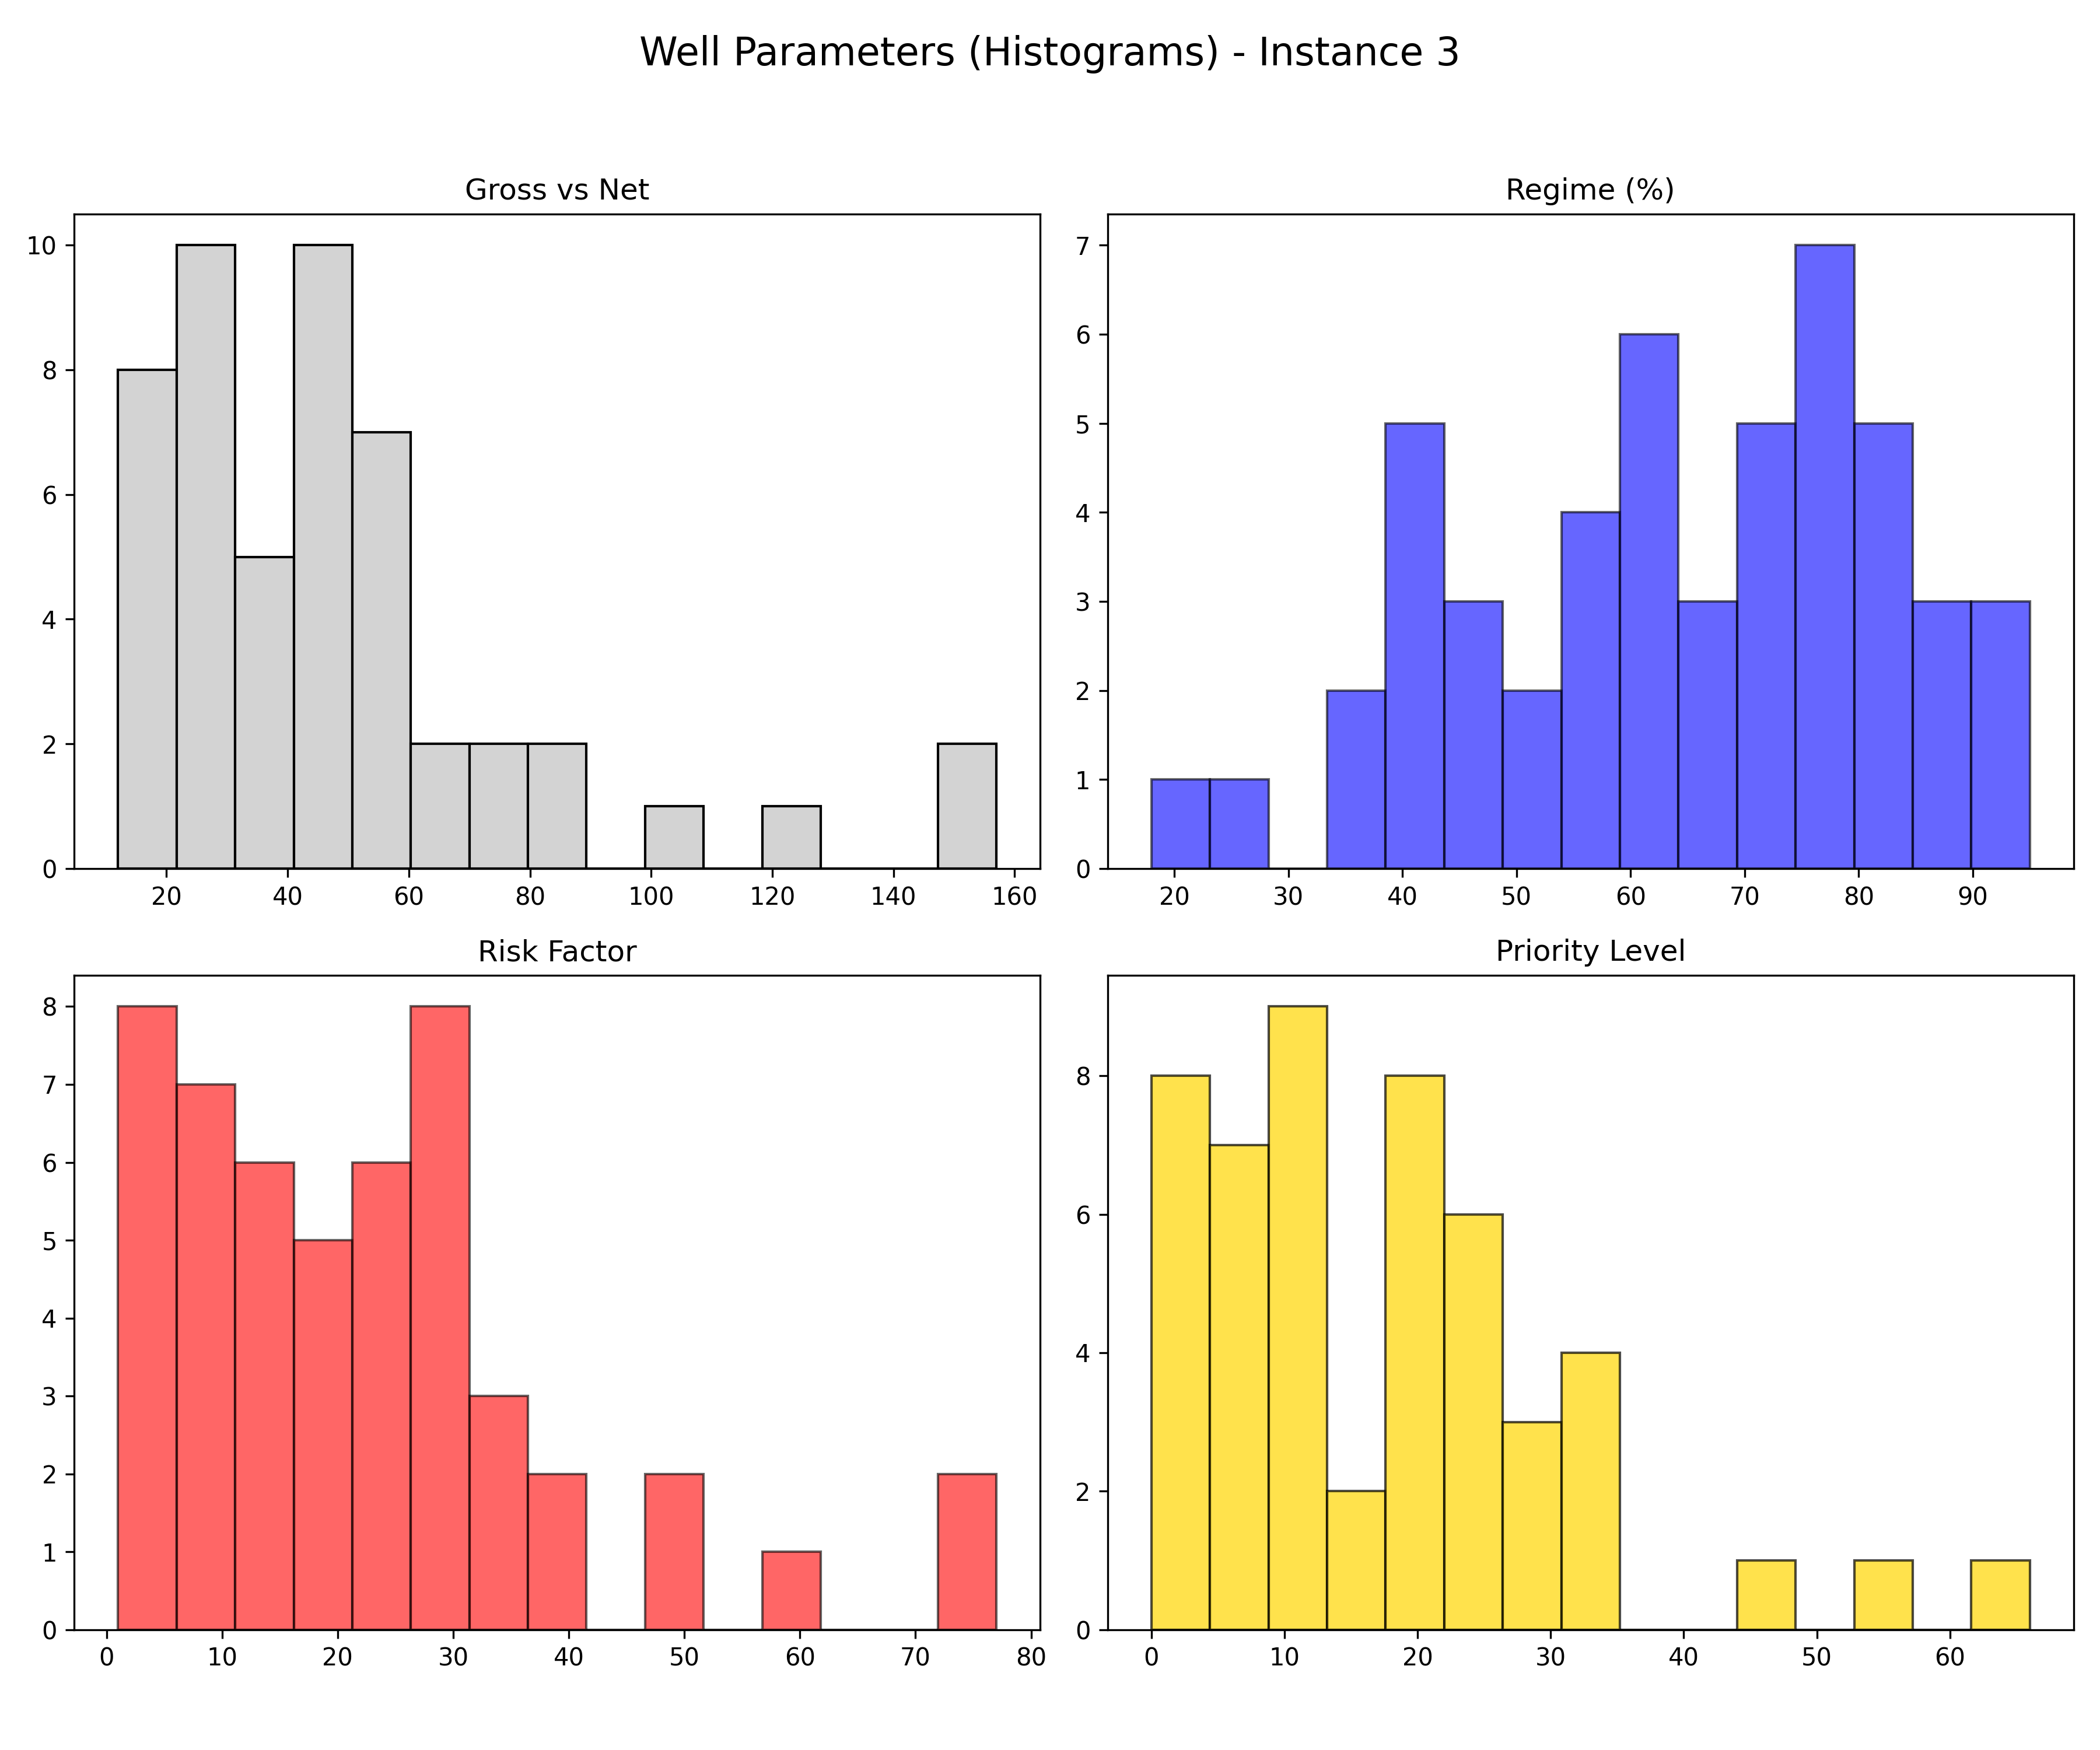
\includegraphics[width=0.75\textwidth]{imagenes/well_hist_1.png}
    \caption{Histograms of well parameters distribution}
    \label{fig:well_hist}
\end{figure}

\begin{figure}
    \centering
    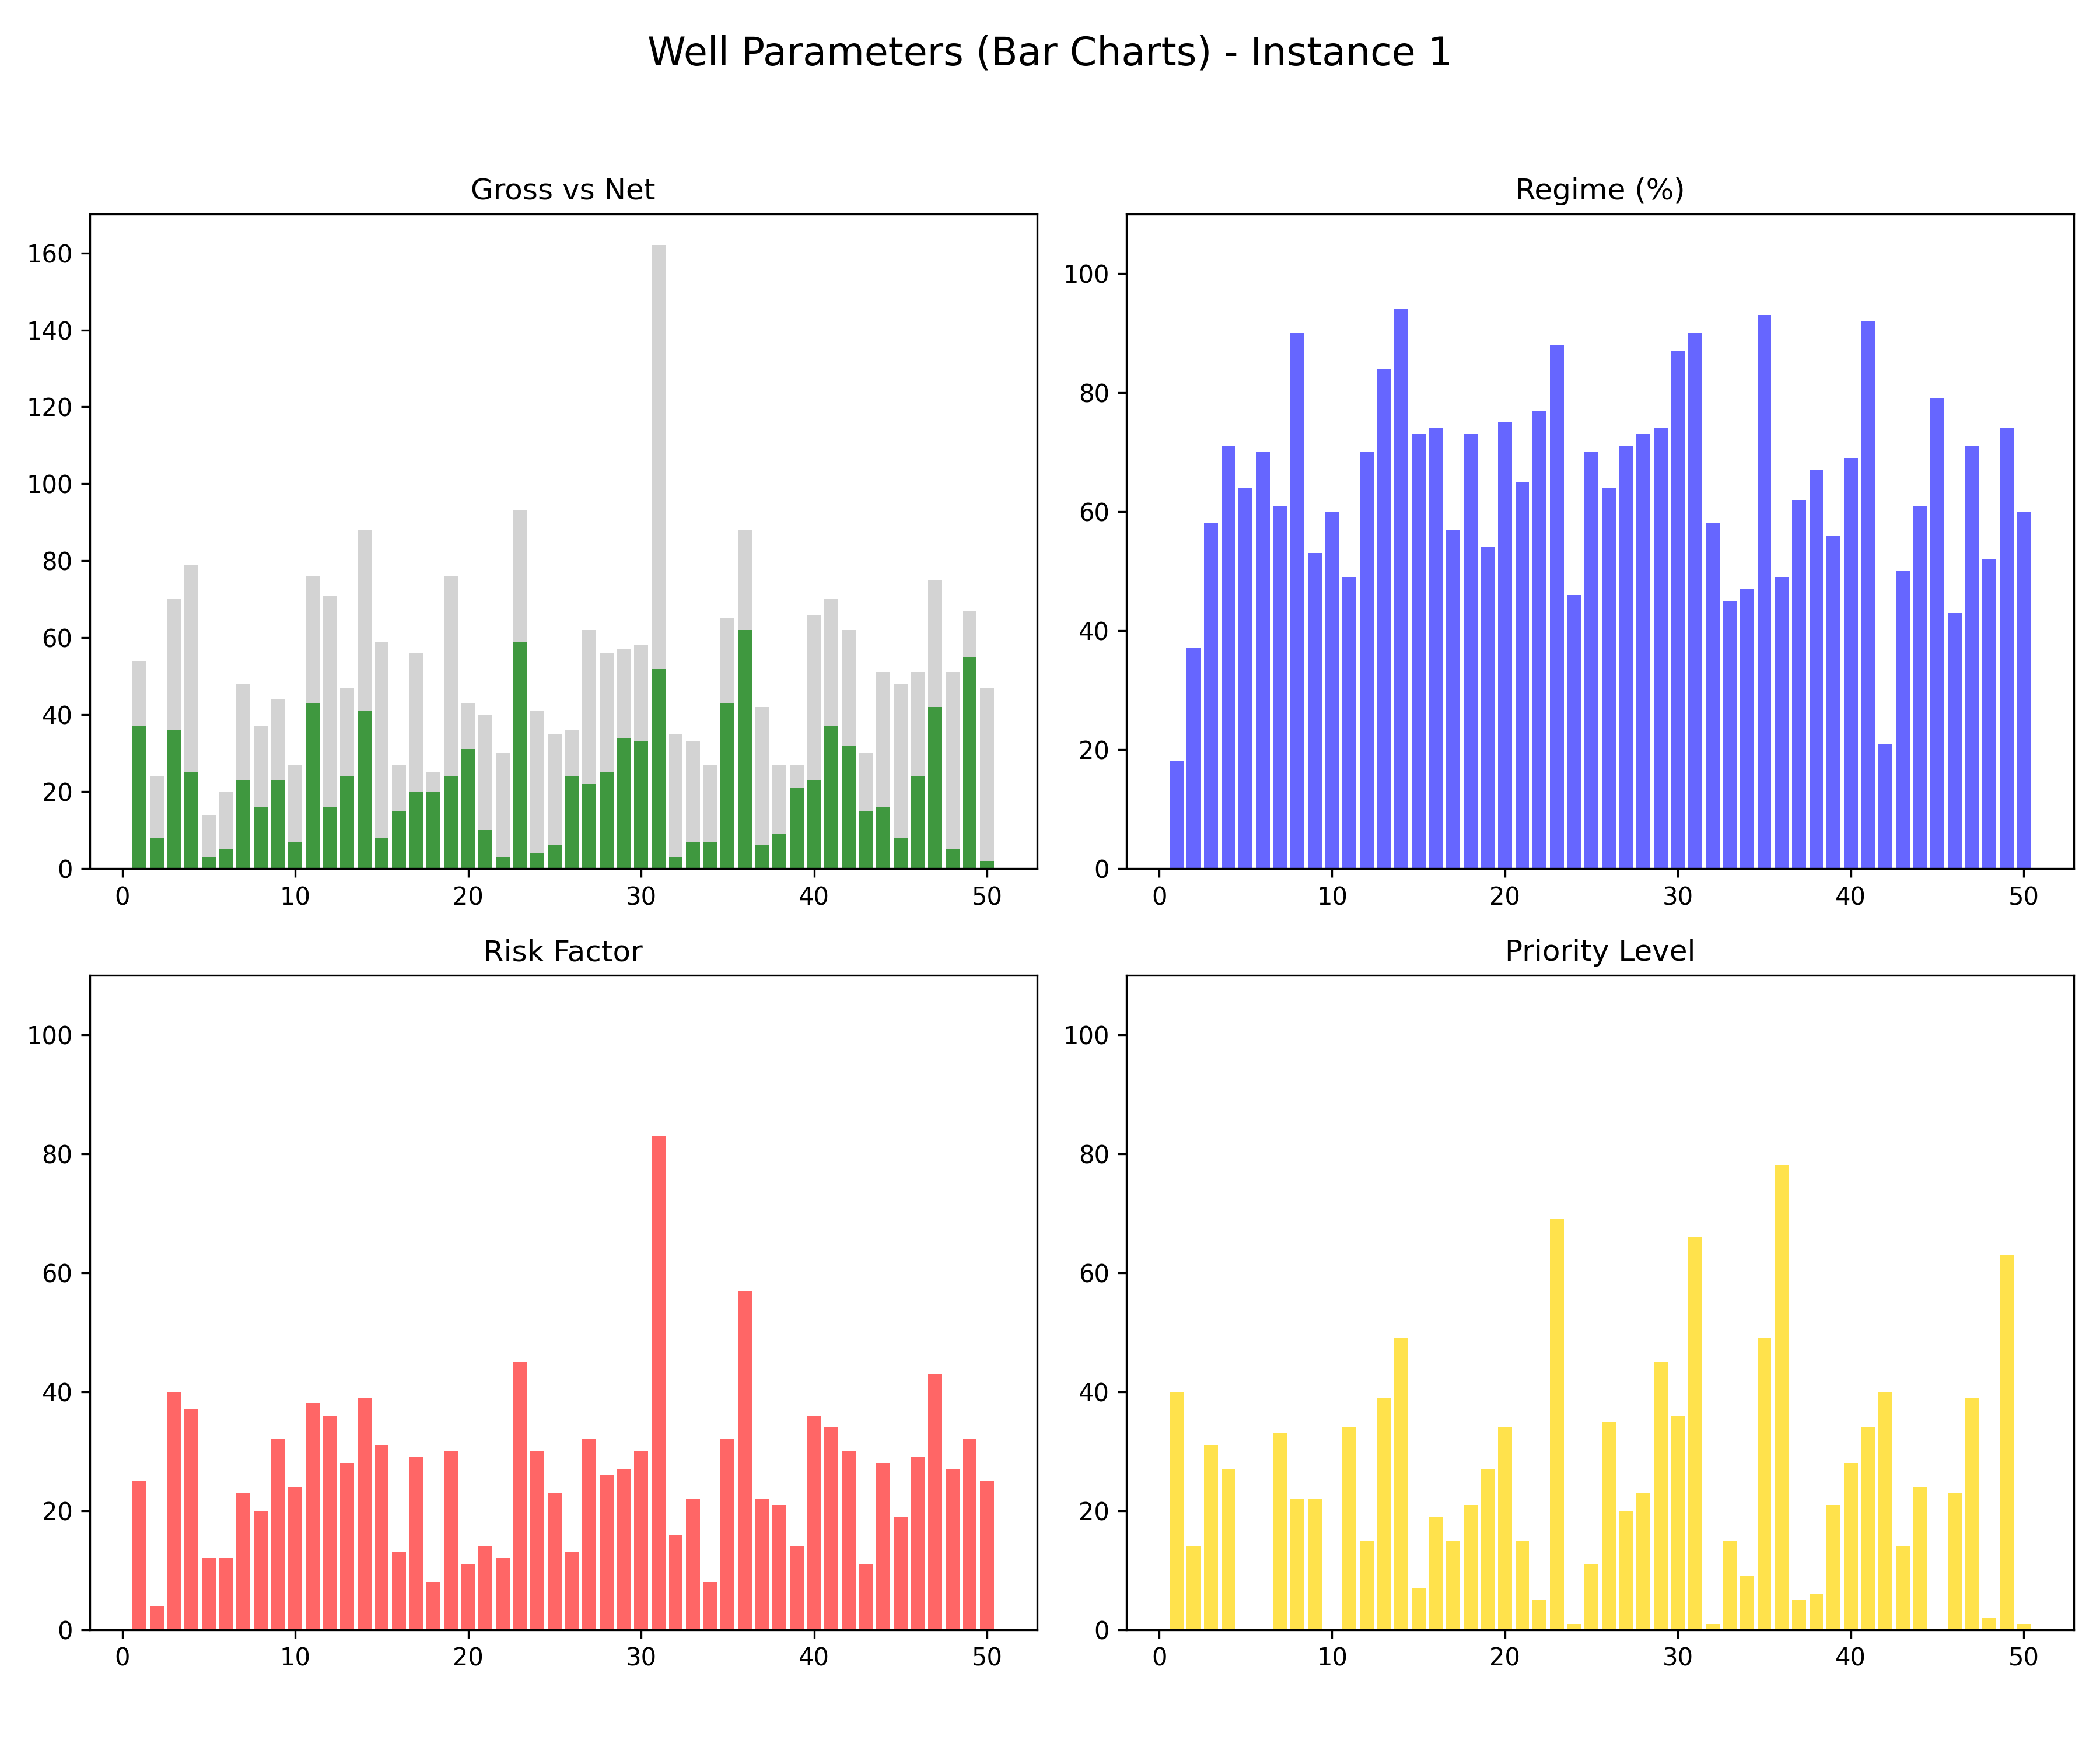
\includegraphics[width=0.75\textwidth]{imagenes/well_bar_1.png}
    \caption{Generated parameters of 50 wells sorted by ID}
    \label{fig:well_dist}
\end{figure}

To represent geographical dispersion and transportation effort in mature oilfields, a synthetic spatial environment is generated over a two-dimensional grid of size $L \times L$. Terrain elevation is produced by combining two components: (i) an interpolated low-resolution random field, and (ii) a configurable set of Gaussian peaks. Let $B(x,y)$ be the normalized interpolated base field and $P(x,y)$ the normalized peak field obtained from $n_{\text{peaks}}$ randomly centered Gaussian kernels. The final elevation is
\[
E(x,y) = A\,\big(\omega_b B(x,y) + \omega_p P(x,y)\big),
\]
where $A$ is the elevation amplitude, and $(\omega_b,\omega_p)=(0.35,0.65)$ in the current implementation. A Gaussian smoothing filter with parameter $\sigma_s$ is then applied. This design makes terrain ruggedness directly controllable through $n_{\text{peaks}}$, $A$, and $\sigma_s$.

Traversal difficulty is induced from topographic slope. Denoting by $\nabla E=(\partial_x E,\partial_y E)$ the discrete gradient (computed with Sobel operators), the slope magnitude is
\[
S(x,y)=\sqrt{(\partial_x E)^2+(\partial_y E)^2},
\]
and the movement cost map is defined as
\[
C(x,y)=1+S(x,y)^{\gamma},
\]
with exponent $\gamma$ controlling how strongly steep terrain is penalized.

Well locations are generated by sampling $n_{\text{clusters}}$ random cluster centers and drawing well coordinates from Gaussian clouds around each center, clipped to the grid domain. The operations center is placed near the geometric center of the field (within a bounded neighborhood) to emulate a central depot.

Road generation is performed in two stages using minimum accumulated-cost paths (MCP). First, primary roads connect each well to the operations center. After each path is created, traversed cells are assigned a very low dynamic cost, which encourages corridor reuse and creates realistic trunk-road consolidation. Second, secondary well-to-well connectors are added to induce loops and alternative routes. Candidate neighbor pairs are filtered by a maximum Euclidean radius and per-well degree limits. For each accepted pair, MCP is solved on a connector-specific map that penalizes reuse of primary-road cells; admissibility is enforced by comparing path cost against a scaled Euclidean threshold. This mechanism improves redundancy while avoiding degenerate overlap with the primary tree-like structure.

Finally, the distance matrix used in the MILP routing component is computed from terrain-based least-cost distances between all nodes (operations center plus wells). Therefore, transportation terms in the optimization model reflect anisotropic travel effort induced by terrain morphology, rather than simple Euclidean proximity.

\begin{figure}
    \centering
    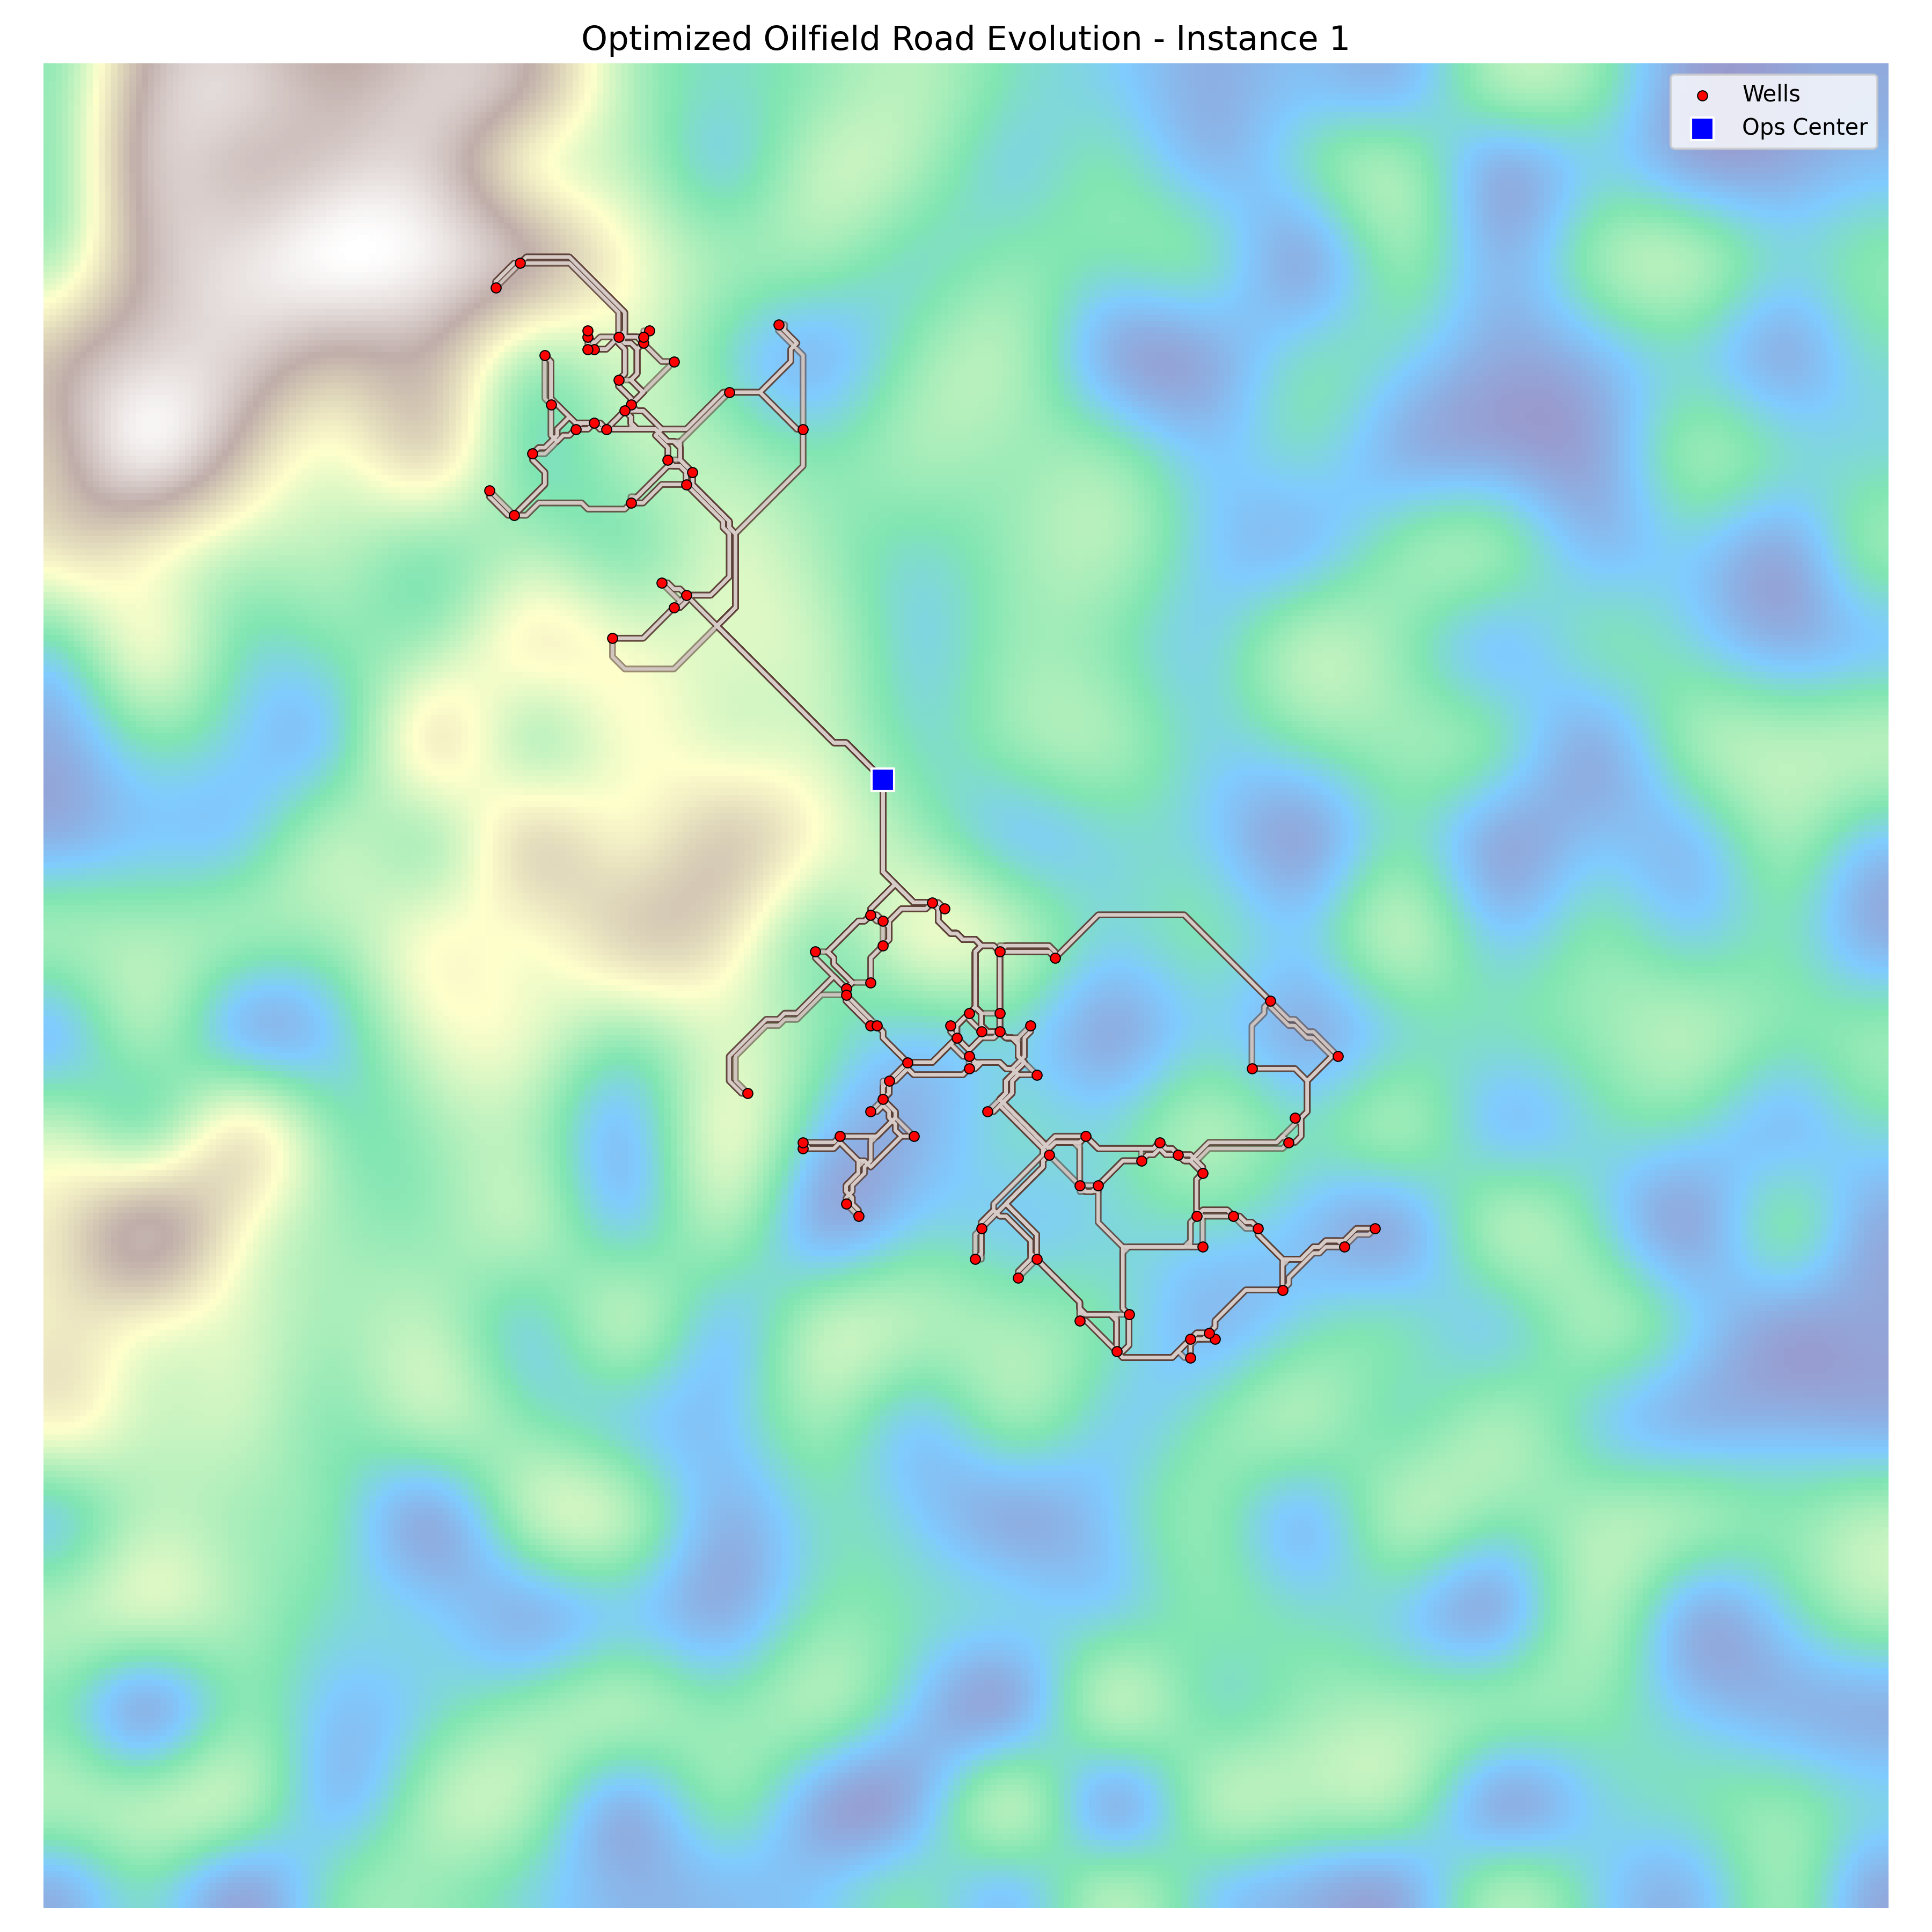
\includegraphics[width=0.75\textwidth]{imagenes/spatial_network_1.png}
    \caption{Procedural generated map of well locations and operations center}
    \label{fig:oil_field_map}
\end{figure}
\section{Results} \label{sec:resultados}

%Below are the results of solving a specific, simplified case, where the distance matrix corresponding to the road diagram in Figure \ref{fig:satelital} was obtained. Parameters for each well were generated randomly using a uniform distribution, assuming a particular initial regime and a target net battery production of $G_{dt}=335 m^3/\text{day}$ after reconfiguration. The distance and production parameters are presented in Tables \ref{tab:uno} and \ref{tab:dos}. The model was solved using the open-source solver SCIP \cite{scipto}, and the Pareto Frontier was generated by minimizing the maximum cumulative loss in the wells while bounding the distance to be traveled. Figure \ref{fig:dos} shows the results obtained. Table \ref{tab:sol} shows the bounded distance to minimize global loss with the new regimes adopted in each well based on the starting point represented by Table \ref{tab:dos}. Values highlighted in bold indicate those wells whose operating regimes were updated.

% \begin{table}[htb]
%     \centering
%     \scalebox{0.55}{
%     \begin{tabular}{|c|c|c|c|c|c|c|c|c|c|c|c|}
% \hline
% Wells&0&1&2&3&4&5&6&7&8&9&10\\
% \hline
%       0&  0	&1025&	927&	459&	955&	1481&	1307&	992&	964&	1332&	1457\\
% 1&1025	&0	&526&	842&	996&	1608&	446&	755&	1087&	1455&	1666\\
% 2&927	&526	&0	&468&	704&	1189&	532&	381&	713&	1081&	1292\\
% 3&459&	842&	468&	0&	496&	1108&	848&	533&	505&	873&	1084\\
% 4&955&	996&	704&	496&	0&	612&	1084&	769&	481&	377&	588\\
% 5&1481&	1608&	1189&	1108&	612&	0&	1466&	1254&	1093&	735&	270\\
% 6&1307&	446&	532&	848&	1084&	1466&	0&	761&	1093&	1461&	1672\\
% 7&992&	755&	381&	533&	769&	1254&	761&	0&	661&	1029&	1240\\
% 8&964&	1087&	713&	505&	581&	1093&	1093&	661&	0&	858&	1069\\
% 9&1332&	1455&	1081&	873&	377&	735&	1461&	1029&	858&	0&	711\\
% 10&1457&	1666&	1292&	1084&	588&	270&	1672&	1240&	1069&	711&	0\\
% \hline

%     \end{tabular}
%     }
%     \caption{Distances among all wells.``Well 0'' is the battery operations center.}
%     \label{tab:uno}
% \end{table}

% \begin{table}[htb]
%     \centering
% \scalebox{0.8} {
% \begin{tabular}{|c|c|c|c|}
% \hline
%    Well ($i$) &	Gross ($G_i$) $m^3/\text{day}$ &	Net ($N_i$) $m^3/\text{day}$ &	Regime ($r_i$) \% \\
% \hline
% 1&	60&	30&	82\\
% 2&	68&	35&	23\\
% 3&	75&	40&	18\\
% 4&	72&	40&	15\\
% 5&	63&	41&	27\\
% 6&	59&	58&	15\\
% 7&	62&	50&	24\\
% 8&	73&	42&	12\\
% 9&	68&	38&	12\\
% 10&	70&	51&	28\\
% \hline
%     \end{tabular}}
%     \caption{Initial parameters for the wells operation.}
%     \label{tab:dos}
% \end{table}

% \begin{table}[htb]
%     \centering
%  \scalebox{0.62}{  
%  \begin{tabular}{|p{1.2cm}|p{1cm}|c|c|c|c|c|c|c|c|c|c|}
%         \hline
%          \multirow{2}{*}{\parbox{1.2cm}{Dist. $m$}} & \multirow{2}{*}{\parbox{1cm}{Loss $m^3/\mbox{day}$}} &\multicolumn{10}{c|}{Well regime \%}\\
%          \cline{3-12}
%          &&1&2&3&4&5&6&7&8&9&10\\
%           \hline
        
%         2400 & 139.5 & 82 & 23 & \textbf{75.5} & \textbf{100} & 27 & 15 & 24 & \textbf{100} & 12 & 28\\
% 2617 & 128 & 82 & 23 & \textbf{94.3} & 15 & 27 & 15 & \textbf{100} & \textbf{100} & 12 & 28\\
% 3376 & 107.7 & \textbf{11.1} & \textbf{100} & \textbf{100} & 15 & 27 & \textbf{100} & \textbf{100} & 12 & 12 & 28\\
% 3857 & 103.8 & \textbf{0} & 23 & \textbf{93.1} & 15 & 27 & \textbf{100} & \textbf{100} & \textbf{100} & 12 & 28\\
% 4329 & 102.4 & \textbf{0} & 23 & \textbf{11.4} & \textbf{100} & 27 & \textbf{100} & \textbf{100} & \textbf{100} & 12 & 28\\
% 4851 & 97.5 & 82 & 23 & \textbf{0} & \textbf{62.8} & 27 & \textbf{100} & \textbf{100} & 12 & 12 & \textbf{100}\\
% 5309 & 90.4 & \textbf{0} & 23 & \textbf{0} & \textbf{62.3} & \textbf{100} & \textbf{100} & \textbf{100} & 12 & 12 & \textbf{100}\\
%         \hline
%     \end{tabular}
%     }
%     \caption{Working regimes for the wells minimizing the traveled distance.}
%     \label{tab:sol}
% \end{table}


\begin{figure}
    \centering
    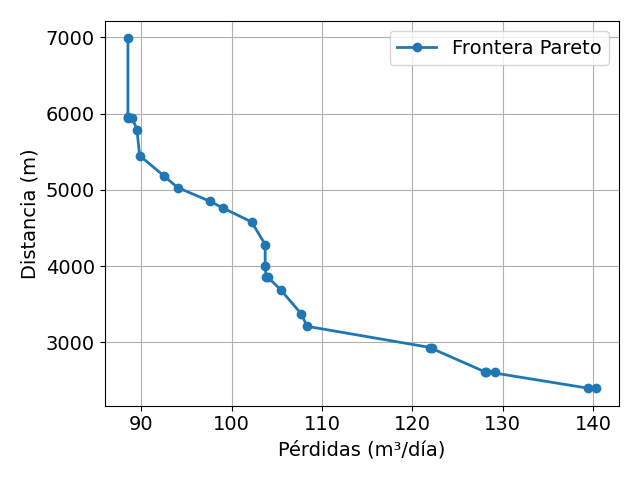
\includegraphics[scale=0.5]{imagenes/plot.png}
    \caption{Pareto's frontier for the example in Section~\ref{sec:resultados}.}
    \label{fig:dos}
\end{figure}
\section{Conclusions} \label{sec:conclusion}

The oil industry is of utmost importance to the global economy and requires constant optimization mechanisms in its various production phases. In particular, oil extraction in southern Argentina requires periodic reconfiguration of various batteries to reduce operating costs, which in many cases is performed manually by an operator. In this ongoing work, an integer linear programming model is presented to schedule the adjustment of the battery regime by modifying the production regimes of the wells along with the itinerary the operator must follow. The computational experiment shows the validity of the model and the feasibility of using it with open-source solvers.Next steps in this line of work will focus on evaluating the complexity of the model and studying alternatives such as heuristics or meta-heuristics for its resolution. We will also seek to scale the application to a set of batteries with a larger number of wells and, on the other hand, consider technical details regarding pumping systems, such as those that impose restrictions on the feasible values of the working regimes.

\bibliography{biblio}

\end{document}
